% vim: set tw=78 sts=2 sw=2 ts=8 aw et ai:

The testbed described in the previous section was used to run test
for low and high bandwidths, starting from 1 Mbps and doubling
up to 1000 Mbps, which is a limit imposed by the Mininet framework itself.
In figures \ref{fig:16mbps-cw} and \ref{fig:16mbps-d}  we can
observe the influence of two major parameters on the throughput for an average
value of 16 Mbps for the bandwidth of each link and no loss on either channel.
The setup is the one that was described in the previous section.

\begin{figure}
  \centering
  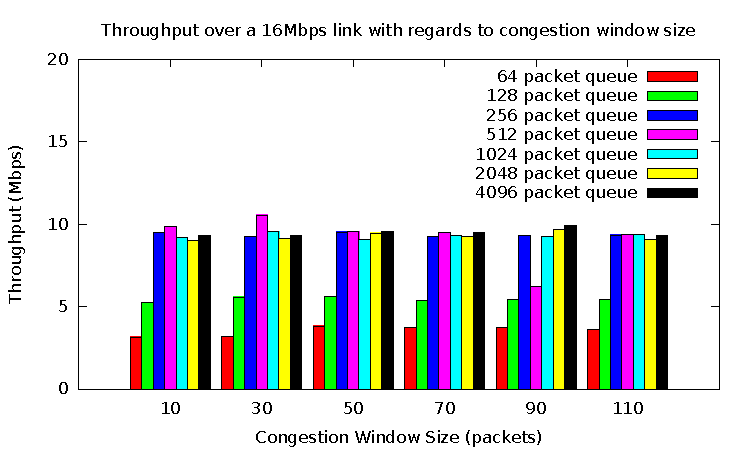
\includegraphics[width=\textwidth]{img/throughput-cwnd-16Mbps}
  \caption{Initial congestion window impact}
  \label{fig:16mbps-cw}
\end{figure}

\begin{figure}
  \centering
  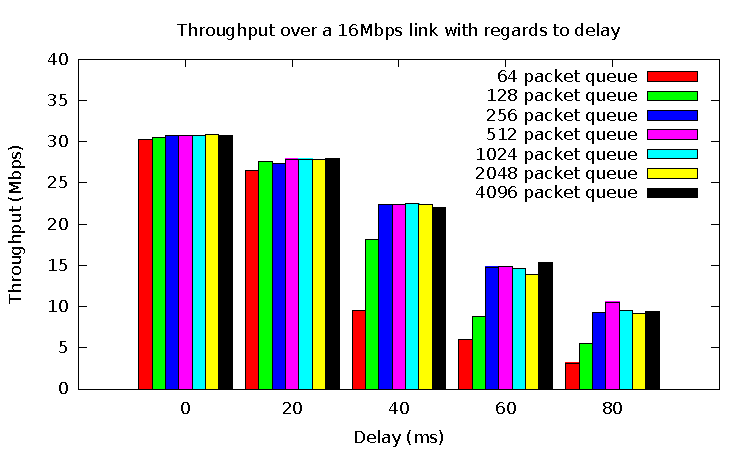
\includegraphics[width=\textwidth]{img/throughput-delay-16Mbps}
  \caption{Channel delay impact}
  \label{fig:16mbps-d}
\end{figure}

Figure \ref{fig:16mbps-cw} shows the impact of the congestion window's initial
size correlated with the receiving queue size. The channel has no losses and
the link delay is 80 milliseconds. It is noticeable that the initial size of
the congestion window does not affect performance too much because MPTCP's
algorithm is adapting it over the course of the data transfer. Throughput is
better for larger receive buffers, but it reaches a ceiling of approximately
10 Mbps because of the sizeable delay.

Figure \ref{fig:16mbps-d} outlines the impact of delay. MPTCP's performance is
close to the maximum possible throughput of 32 Mbps regardless of the receive
buffer when there is zero delay. The performance expectedly decreases when delay
is larger and we notice that the receive buffer size starts to influence
throughput. That is because the size of the receive buffer is conditioned by the
bandwidth-delay product as it was mentioned in Section \ref{sec:related}.
As the delay increases, small receive buffers lead to poor channel utilization
and consequently the throughput is reduced.

\begin{figure}
  \centering
  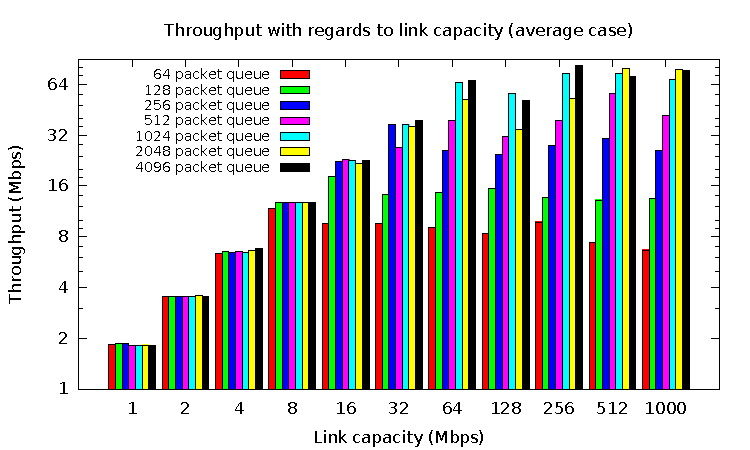
\includegraphics[width=\textwidth]{img/throughput-bdw-avg}
  \caption{Link capacity impact with average delay}
  \label{fig:bdw-avg}
\end{figure}

\begin{figure}
  \centering
  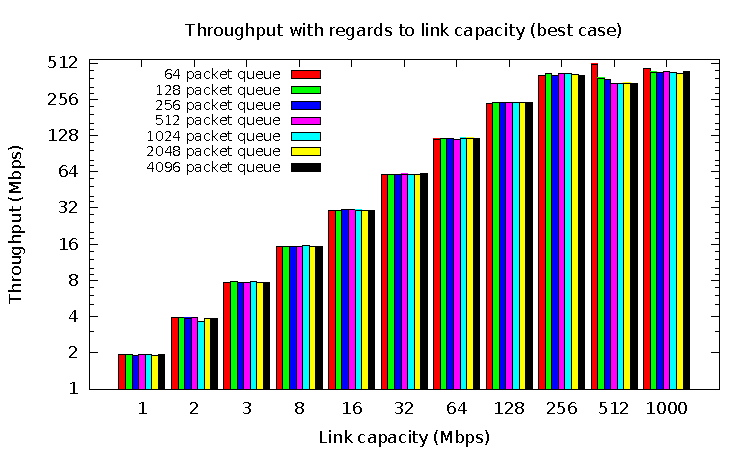
\includegraphics[width=\textwidth]{img/throughput-bdw-max}
  \caption{Link capacity impact with no delay}
  \label{fig:bdw-max}
\end{figure}

As mentioned in Section \ref{sec:tcp-link}, the impact of the available link
capacity is undeniably significant. Figure \ref{fig:bdw-avg} outlines the
throughput between two nodes when the initial congestion window is of 50
packets, and with an average delay of 40 milliseconds, for various bandwidth
and receiver queue size. It is worth underlining the fact that, as link
capacity increases, so does the bandwidth-delay product. Therefore, for links
with capacity of 16Mbps and above, we notice the same behavior of poor channel
utilization for small receiver queues. The difference is most visible for the
gigabit link.

\begin{figure}
  \centering
  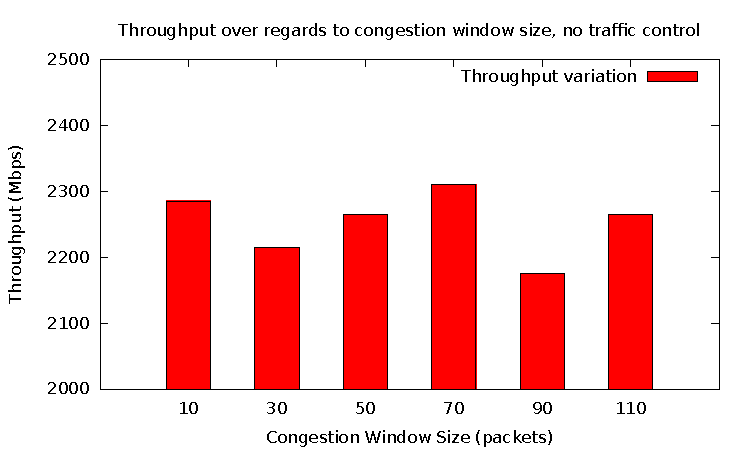
\includegraphics[width=\textwidth]{img/throughput-cwnd-notc}
  \caption{Throughput without overhead associated with traffic control}
  \label{fig:cwnd-notc}
\end{figure}

While attempting to isolate the exact parameters that lead to ideal MPTCP
performance, we have tested how throughput evolves when delay is factored
out. By setting the delay to 0 milliseconds the framework sends packets as
quick as it can generate them. As it can be observed in Figure
\ref{fig:bdw-max}, MPTCP is able to fully make use of both links and thus the
throughput is double the capacity of a single link. However, as we tested with
higher bandwidths, namely 256 Mbps and above, we noticed that the throughput
was somehow capped.

After looking into the way Mininet models parametrized links, we have found
that it relies on the tc utility to perform traffic shaping. While the ability
to control several aspects of the link between two nodes was extremely useful
towards our tests, traffic shaping is a costly operation in terms of
computational power. Given the fact that our testbed is represented by a
virtual machine which itself employs to process and network namespaces, we
conclude that the throughput cap manifests because the processing power of the
virtual machine is not sufficient to process packets as quickly as it would be
necessary to reach throughputs in the realm of gigabit networking. This is
perhaps the reason why Mininet introduces an upper bound to the link capacity
that can be used on a parametrized link.

In order to validate the claim that CPU limitations lead to throughput
capping, we have performed another test in which we sacrifice the ability
to configure link features in order to properly get a sense of how much
data can MPTCP pass between two nodes if given enough resources. To this end,
Figure \ref{fig:cwnd-notc} presents throughput over links without employing
traffic shaping. We are still able to control the initial congestion window,
but nothing more. In this scenario, we notice that regardless of the initial
congestion window, MPTCP is able to reach throughputs of over 2 Gbps, which
highlights the significant effect of traffic shaping. Nevertheless, while the
maximum throughput is heavily affected by link parametrization, the previously
described MPTCP behavior is still relevant, as CPU limitations do not manifest
until higher rates are attempted.

